\begin{pastexam}[label={px:ntu-107-dsa-02}]{臺大資工所 107 學年度 第 II 題}
（單選；答錯倒扣當題分數）

(8 points) In a \textit{min-heap} stored in an array, please answer the following questions after these 11
numbers have been inserted: $12,8,23,21,6,1,7,25,24,22,26$.
\begin{enumerate}[label=\textbf{\arabic*.}, start=8]
\item (2 points) What is the height of the heap? (A) 2 (B) 3 (C) 4 (D) 5
\item (3 points) What is the value of the node at index 3? (A) 1 (B) 6 (C) 7 (D) 8
\item (3 points) What is the value of the left child of the node with value 12? (A) 22 (B) 24
(C) 25 (D) 26
\end{enumerate}
\end{pastexam}

\begin{pastsoln}
答案：8.~(B) 3\quad 9.~(B) 6\quad 10.~(A) 22。

\textbf{題意。} 「inserted」照字面讀成一個一個插入（每次放在陣列最後再上浮），不是把 $11$ 個數一次
放好再由下而上建堆積（那樣做得到 $[1, 6, 7, 21, 8, 23, 12, 25, 24, 22, 26]$，$12$ 在位置 $7$ 是葉節點，
第 10 題就問不下去了）。 陣列從 $1$ 開始（CLRS 的寫法；第 9 題的選項也只有這樣讀才對得上，見下）。
高度照 CLRS 的定義數\textbf{邊}，見第 8 題。

\textbf{插入過程}（最小堆積的上浮：比父節點小就交換，資結書第~8.1~節）：
\begin{center}
\small
\begin{tabular}{rll}
\toprule
插入 & 過程 & 之後的陣列 \\
\midrule
12 & 放在位置 1 & $[12]$ \\
8 & 位置 2；$8 < 12$，交換 & $[8, 12]$ \\
23 & 位置 3；$23 > 8$，不動 & $[8, 12, 23]$ \\
21 & 位置 4；父節點 $12$，不動 & $[8, 12, 23, 21]$ \\
6 & 位置 5；$6 < 12$ 換到位置 2；$6 < 8$ 換到根 & $[6, 8, 23, 21, 12]$ \\
1 & 位置 6；$1 < 23$ 換到位置 3；$1 < 6$ 換到根 & $[1, 8, 6, 21, 12, 23]$ \\
7 & 位置 7；父節點是位置 3 的 $6$，不動 & $[1, 8, 6, 21, 12, 23, 7]$ \\
25 & 位置 8；父節點 $21$，不動 & $[1, 8, 6, 21, 12, 23, 7, 25]$ \\
24 & 位置 9；父節點 $21$，不動 & $[\ldots, 25, 24]$ \\
22 & 位置 10；父節點是位置 5 的 $12$，不動 & $[\ldots, 25, 24, 22]$ \\
26 & 位置 11；父節點 $12$，不動 & $[1, 8, 6, 21, 12, 23, 7, 25, 24, 22, 26]$ \\
\bottomrule
\end{tabular}
\end{center}
最後的堆積（節點旁的小字是陣列位置）：
\begin{center}
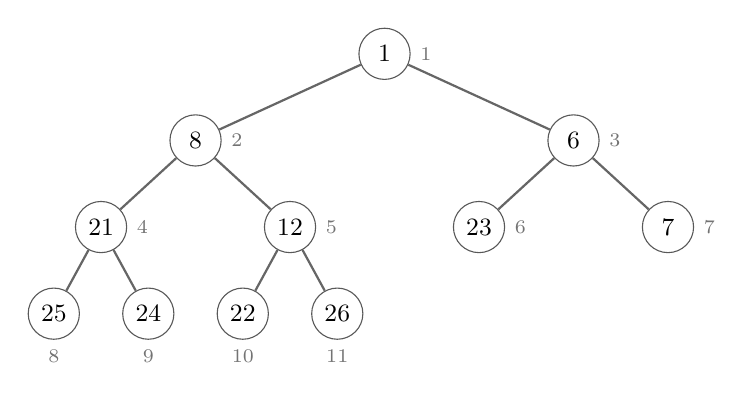
\begin{tikzpicture}[
    hn/.style={circle, draw=black!65, line width=0.4pt, minimum size=6.5mm, inner sep=0pt, font=\small},
    level distance=11mm, edge from parent/.style={draw=black!60, thick},
    level 1/.style={sibling distance=48mm}, level 2/.style={sibling distance=24mm},
    level 3/.style={sibling distance=12mm},
    ix/.style={font=\scriptsize, text=black!55}]
\node[hn, label={[ix]right:1}] {1}
    child {node[hn, label={[ix]right:2}] {8}
        child {node[hn, label={[ix]right:4}] {21}
            child {node[hn, label={[ix]below:8}] {25}}
            child {node[hn, label={[ix]below:9}] {24}}}
        child {node[hn, label={[ix]right:5}] {12}
            child {node[hn, label={[ix]below:10}] {22}}
            child {node[hn, label={[ix]below:11}] {26}}}}
    child {node[hn, label={[ix]right:3}] {6}
        child {node[hn, label={[ix]right:6}] {23}}
        child {node[hn, label={[ix]right:7}] {7}}};
\end{tikzpicture}
\end{center}

\textbf{8. (B) 3。} $11$ 個節點的完整二元樹有 $4$ 層（第 $4$ 層是位置 $8$--$11$）。 CLRS 的高度數
邊，是根到最深葉節點的邊數 $\lfloor \lg 11 \rfloor = 3$。 資結書的高度數節點
（資結書第~7~章），那樣算是 $4$，就會選 (C)。 這份考卷用的是 CLRS 的名詞，這裡取 CLRS 的
定義；作答時最好寫一句「高度以邊數計」。 (A) 2、(D) 5 在兩種定義下都不對。

\textbf{9. (B) 6。} 陣列從 $1$ 開始，位置 $3$ 是根的右子節點 $6$。 如果從 $0$ 開始，$A[3] = 21$，
不在選項裡，所以題目的陣列是從 $1$ 開始。 (A) 1 是位置 $1$，(D) 8 是位置 $2$，(C) 7 是位置 $7$。

\textbf{10. (A) 22。} $12$ 在位置 $5$，左子節點在位置 $2 \cdot 5 = 10$，是 $22$；右子節點在位置
$11$，是 $26$（選項 (D)）。 (B) 24、(C) 25 是 $21$ 的子節點。
\end{pastsoln}
